\begin{frame}{Opérations sur les noms de fichiers (\texttt{ln (-s)}, \texttt{rm}, \texttt{mv})}
    \texttt{ln f (-s)} : création d'un lien physique (symbolique).
    
    \texttt{rm f -f} : efface le fichier de nom f
    
    \texttt{mv f1 f2} : renomme le fichier de nom f1 en f2
    \pause
    
    \subtt{Exemple}
    
    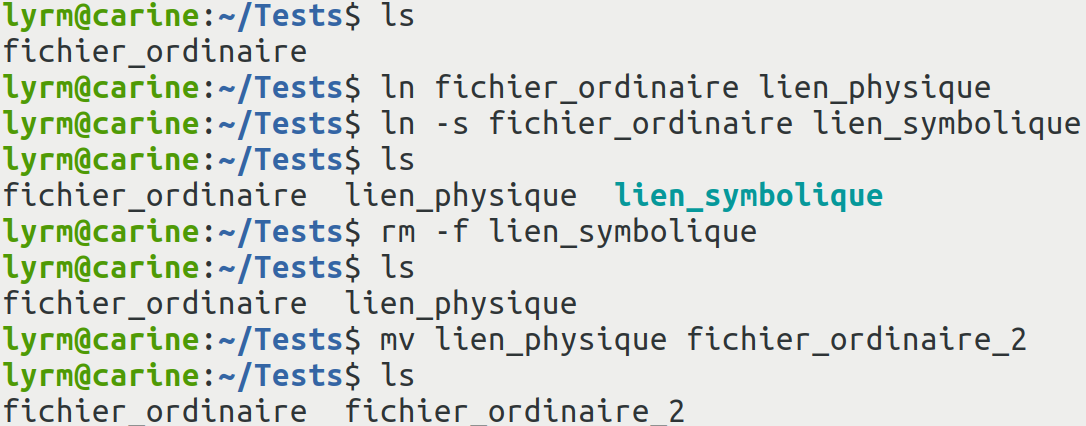
\includegraphics[width=0.7\textwidth]{slides/images/shell_ln_rm_mv.png}
    \pause 
    
    Facile : ce sont des fonctions \texttt{Unix} existantes.
\end{frame}

\begin{frame}[fragile]{Opérations sur les noms de fichiers (\texttt{ln (-s)}, \texttt{rm}, \texttt{mv})}
    \begin{lstlisting}
        (* Efface un fichier *)
        val unlink : string -> unit
        
        (* Renomme un fichier *)
        val rename : string -> string -> unit
        
        (* Creer un lien physique *)
        val link : ?follow:bool -> string -> string -> unit
        
        (* Creer un lien symbolique *)
        val symlink : string -> string -> unit
        
        (* Lit le contenu d'un lien symbolique *)
        val readlink : string -> string
    \end{lstlisting}
\end{frame}

\begin{frame}[fragile]{Opérations sur les noms de fichiers (\texttt{ln (-s)}, \texttt{rm}, \texttt{mv})}
    \begin{lstlisting}
        let exec_cmd cmd = match cmd with 
          | Cat files -> ...
          
          | Ln (source, dest, symbolic) ->
            if symbolic then Unix.symlink source dest 
            else Unix.link source dest

          | Mv (source, dest) -> Unix.rename source dest

          | Rm (filename, recursive) ->
            if recursive then failwith "todo" 
            else Unix.unlink filename
            
          | ... -> ...   
    \end{lstlisting}
\end{frame}

\begin{frame}{Opérations sur les répertoires (\texttt{mkdir (-m int)}, \texttt{rm -r}, \texttt{ls})}
     \texttt{mkdir dir (-m int)} : créer un répertoire avec les permissions définies par l'option \texttt{-m}.

     \texttt{rm -r dir} : efface le répertoire nommé \texttt{dir} et son contenu .
    
    \texttt{ls dir} : liste le contenu du répertoire \texttt{dir} ou du répertoire courant par défault sur la sortie standard.
    \pause
    
    \subtt{Exemple}
    
    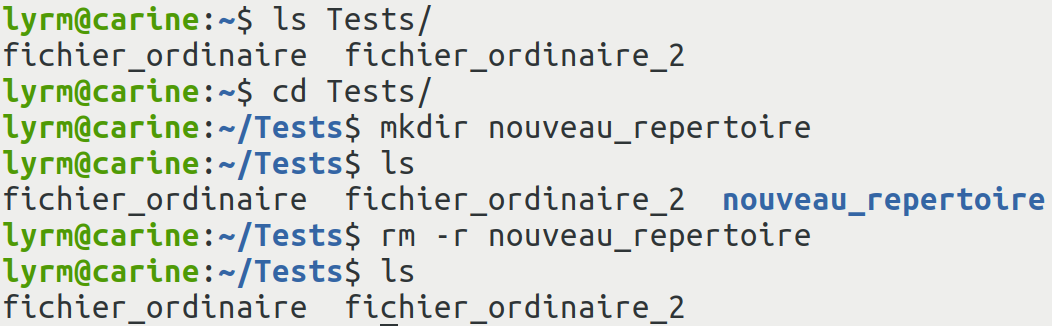
\includegraphics[width=0.8\textwidth]{slides/images/shell_mkdir_rm_ls.png}

\end{frame}

\begin{frame}[fragile]{Opérations sur les répertoires : \texttt{mkdir (-m int)}, \texttt{rm -r}}
    \subtt{Fonctions Unix :}
     \begin{lstlisting}
          type file_perm = int (* ex : 0o777 *)
          val mkdir : string -> file_perm -> unit
          val rmdir : string -> unit
     \end{lstlisting}
    \pause
    \subtt{Implémentation :}
    \begin{lstlisting}
        let exec_cmd cmd = match cmd with
          | Rm (filename, recursive) ->
            if recursive then Unix.rmdir filename
            else Unix.unlink filename
          | Mkdir (filename, perm_opt) -> (* Note : Le parseur ajoute "0o" devant la perm (666 ici) ([mkdir name -m 666])  *)
            let perm = match perm_opt with None -> 0o775 | Some p -> p in
            Unix.mkdir filename perm
          |  ... -> ...   
    \end{lstlisting}
\end{frame}
     
\begin{frame}[fragile]{Opérations sur les répertoires : \texttt{ls}}
    \subtt{Fonctions Unix :}
    \begin{lstlisting}[basicstyle=\scriptsize\ttfamily]
          type dir_handle             (* descripteur de lecture *)
          val opendir : string ->  dir_handle
          val readdir : dir_handle -> string  (* lit une entree *)
          val closedir : dir_handle -> unit
    \end{lstlisting}
    
    \subtt{Boucle de lecture des entrées du répertoire}
    \begin{lstlisting}[basicstyle=\scriptsize\ttfamily]
    let read_dir dirname =
      let rec loop dir_handle acc =
        try  
          let nfile = Unix.readdir dir_handle in
            loop dir_handle (nfile :: acc)
        with End_of_file -> acc in
        
      let dir_handle = Unix.opendir dirname in (* Ouverture *)
      let files = loop dir_handle [] in          (* Lecture *)
      Unix.closedir direname;                  (* Fermeture *)
      files
    \end{lstlisting}
\end{frame}

\begin{frame}[fragile]{Opérations sur les répertoires : \texttt{ls}}
        \begin{lstlisting}
    let exec_cmd cmd = match cmd with
        | Ls diropt ->
          let dirname = match diropt with 
            | None -> Filename.current_dir_name 
            | Some d -> d  in
          (* Lecture *)
          let files = read_dir dirname in
          (* Filtrage *)
          let files =  List.filter
              (fun file ->
                not (file = Filename.parent_dir_name || 
                     file = Filename.current_dir_name))
              all_files in
          (* Concatenation *)
          let files = String.concat "\t" files in
          (* Ecriture sur la sortie standard *)
          write_stdout (files ^ "\n")
        | ... -> ...
        \end{lstlisting}
\end{frame}

\begin{frame}[fragile]{Opérations sur les répertoires : \texttt{ls}}

    La fonction d'écriture sur la sortie standard ressemble beaucoup à celle vue précédemment :
    \begin{lstlisting}
        let write_stdout text =
          (* Conversion en bytes *)
          let text = Bytes.of_string text in
          (* Taille max du bloc d'ecriture *)
          let max_len = 8192 in
          (* boucle d'ecriture *)
          let rec loop ind to_write =
            let len = min max_len to_write in
            let written = Unix.single_write Unix.stdout text ind len in
            if written = max_len then
              loop (ind + written) (to_write - written)
          in
          loop 0 (Bytes.length text)
    \end{lstlisting}
\end{frame}

\begin{frame}[fragile]{Opérations sur les répertoires : \texttt{ls}}
    \subtt{Ajouter l'option \texttt{-i} pour \texttt{ls}}
    
    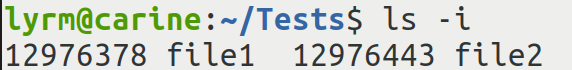
\includegraphics[width=0.5\textwidth]{slides/images/shell_ls_inode.png}
    
    \subttt{Fonctions disponibles : }
    \begin{lstlisting}
    (* Information sur le fichier *)
    val stat : string -> stats
    (* Comme [stat] avec un descripteur de fichier *)
    val fstat : file_descr -> stats
    (* Donne l'information sur un lien symbolique *)
    val lstat : string -> stats
    \end{lstlisting}
    
\end{frame}

\subsection{Gestion des erreurs Unix et boucle principale de lecture}

\begin{frame}[fragile]{Boucle principale de lecture : premier essai}

    \begin{lstlisting}
     let minishell () =
      try
        while true do
          let cmd_line = Stdlib.input_line Stdlib.stdin in
          try
            let cmd : Command.t = Parser.parse cmd_line in
            Command.exec_cmd cmd
          with
          | Parser.Parsing_error err -> Parser.print_error err
          | Parser.Empty_line -> ()
        done
      with End_of_file -> ()
    \end{lstlisting}

\end{frame}

\begin{frame}[fragile]{Gestion des erreurs}
    
    \begin{lstlisting}
         Unix.handle_unix_error : ('a -> 'b) -> 'a -> 'b
    \end{lstlisting}
\end{frame}
